%************************************************
\chapter{Problem Statement}\label{ch:problemstatement}
%************************************************

This section will further define the problem and derive formal requirements to event subscription mechanisms

\section{Motivating Examples}
- one example for independent. The subscription does not depend on a prior precess result, the subscription can be done even before process instantiation

- one example for a process that uses an intermediate event that depends (subscription-wise) on the result of a previous step in the process.

==> If the event occurs at a certain time, the process gets delayed unnecessarily or even run into a deadlock

\section{Event Occurrence Scenarios}
Given the motivating examples, I am deriving a generic set of event occurrence scenarios. Each of these scenarios can occur in the real world and process implementations need to be capable of handling them to avoid negative effects.

\paragraph{Time of event occurrence}

The most important variable to consider is the time of event occurrence. According to the BPMN specification, it is possible to catch an event if it occurs after the event element is enabled. As shown before, it is often impossible to control occurrence time and events do occur outside of these time windows.
We specify the possible event occurrence times in relation to the life cycle of a process that utilizes a BPMN Intermediate Event \todo[inline]{ref process lifecycle}.
\begin{figure}[]
	\myfloatalign
	{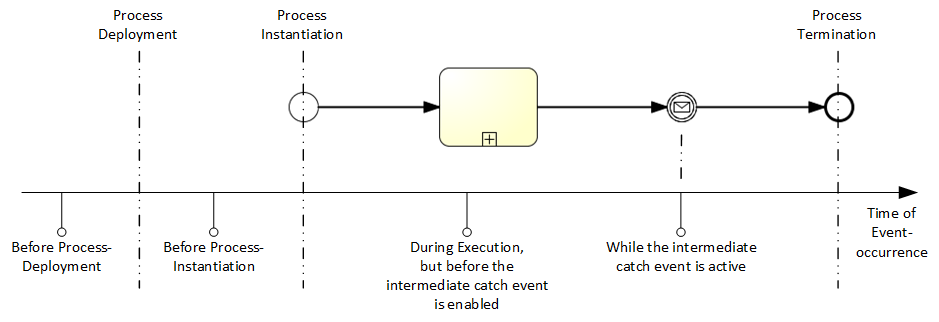
\includegraphics[width=1\linewidth]{chapters/requirements/timeline-event-occurrence.png}}
	\caption{Possible event occurrence times in relation to a process execution life cycle}\label{fig:occurrence-timeline}
\end{figure}

\autoref{fig:occurrence-timeline} shows the life cycle steps of a process and an instance from the deployment of the process until the undeployment and uses a timeline to illustrate that an event might occur at any time during this cycle. More precisely, an event is always considered to occur before or after a life cycle step or in between two consecutive steps.
\todo[inline]{How about system-deployment/process engine start and process undeployment? show in illustration, but say in text that we simplify this for now. after undeployment is essentially before deployment of a new process; Before Engine start is also before pr. deployment and we presume that an engine is running and does not stop.}

Given the relevant life cycle steps, \textit{process deployment}, \textit{process instantiation} and \textit{Event enablement}, the following four occurrence phases are distinguished in this work:
\begin{aenumerate}
	\item O1 Before Process deployment
	\item O2 Between Process deployment and process instantiation
	\item O3 Between Process instantiation and the enabling of the BPMN event
	\item O4 After the enabling of the BPMN event
\end{aenumerate}\label{def:occurrence-times}

\todo[inline]{add a back reference to the examples? In example XY, events can occur before... whereas in example...}

For a flexible and efficient use of events in business processes, it must be possible to use events that occur in any of these phases.
To make sure that an event can be caught, no matter at which time during the phase it occurs, the subscription to the CEP platform must happen at the beginning of the occurrence phase.
It follows that the event subscription must be possible at system start, at process deployment, at process instantiation, at any time during process execution and when the BPMN Event element is enabled.

\paragraph{Event Subscription Dependencies}
It is important to note that the subscription to an event source can depend on additional context information or process data. This can be a severe limitation to the possible subscription time.
\todo[inline]{ref to process model} shows a logistics process that uses event data about the GPS position of a certain truck to keep the estimated time of arrival of the transport updated. Whenever it receives an updated GPS position, the ETA is re-calculated; once the \textit{arrival}-event has been received, the process finishes.

\todo[inline]{this example is not good, because we are not interested in a gps event that occurs earlier. Find an example where you would like earlier events, but subscription is not possible}

Before the subscription to that specific truck gps event can happen, the process must determine the \textit{truckId} to use in the event query. Only when the \textit{truckId} is available, the subscription can be executed. This example illustrates how a query filter expression can depend on context data, but it might as well be the event source itself that differs depending on the particular execution.

\todo[inline]{there could be an xor gateway and following two different events and only one of them can get executed}

\todo[inline]{solution would be to listen to all gps, but potentially too much data. Decision must be made cautiously! <= Where should I mention this? maybe later in the concept}


\section{Requirements Definition}
The previous sections have exemplified how the execution semantic offered by the BPMN specification limits users in the use of events in business processes. Now these shortcomings are formalized into an additional set of requirements that must be met by a process execution environment to enable event handling in the extended set of event occurrence scenarios.
The formal requirements will later be used to evaluate the capabilities of current Process Management Solutions and to develop a new concept to handling event subscription in business processes. \todo[inline]{ref to chapters}

\paragraph{R1: Flexible Event Subscription Time\newline}

\textit{R1.1: Explicitness}: 
For each event that is used in a business process, it must be possible to derive the time of event subscription from the process model. The time of subscription may either be explicitly stated or defined implicitly.

\textit{R1.2: Flexibility}: 
The time of subscription can be influenced to catch events according to any of the event occurrence scenarios O1, O2, O3, O4. In other words, the process model defines the earliest acceptable time for an event occurrence to be considered in the process execution. The necessary options are \textit{since system start}, \textit{since process deployment}, \textit{since process instantiation}, from an arbitrary but \textit{explicit time during process execution}, or \textit{since enabling of the Event Process Element}.

\paragraph{R2: Automatic Subscription Handling\newline}

\textit{R2.1: Subscription}
The subscription to event sources is handled implicitly by the process execution environment as defined by the process model.

\textit{R2.2: Removal of Subscription}
The removal of a subscription from the system is handled automatically as soon as a subscription becomes unnecessary.

\paragraph{R3: Event Buffering\newline}
To make all events since the subscription time available during process execution, matching events need to be stored temporarily.

\todo[inline]{buffer policies and scope?}